   
        
        \begin{ledgroupsized}[r]{120mm}
        \footnotesize 
        \pstart        
        \noindent\textbf{\"{U}berlieferung:}  
        \pend
        \end{ledgroupsized}
      
       
              \begin{ledgroupsized}[r]{114mm}
              \footnotesize 
              \pstart \parindent -6mm
              \makebox[6mm][l]{\textit{L}}Konzept: LH XXXVIII Bl. 138. 1 Bl. 17 x 18 cm. 1 S. Papier gleichm\"{a}ßig beschnitten, R\"{u}ckseite leer. Datierung in der linken oberen Ecke. Zeichnung und Nebenrechnung am linken Rand.\\Cc 2, Nr. 966 C \pend
              \end{ledgroupsized}
        \vspace*{8mm}
        %\pstart 
        \normalsize
      \begin{center}[138 r\textsuperscript{o}] Maji 1675\\ Probleme:\end{center} \pstart \textso{Un bâton estant fich\'{e} dans le fonds d'un foss\'{e} plein d'eau, et sortant tant soit peu hors de l'eau juger de la profondeur de l'eau ou du foss\'{e} sans tirer le bâton et sans en s\c{c}avoir la longueur, pourveu qu'on aye la libert\'{e} de le remuer.}\pend \pstart \textso{Ou si vous voulez une sonde estant jett\'{e}e }\textso{ dans la mer et touchant fonds, juger de la profondeur de la mer, sans retirer la sonde, et sans s\c{c}avoir la longueur de la corde.}\edtext{}{\lemma{\textso{corde}.}\Afootnote{\textit{Markierung durch Anf\"{u}hrungszeichen am linken Rand.}}} \pend \pstart Soit le bâton ou la sonde, \textit{AB} touchant fonds au bout \textit{B} sortant de
%  Zeitz auskommentiert       \begin{wrapfigure}{l}{0.22\textwidth}          
%         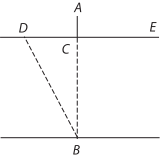
\includegraphics[width=0.22\textwidth]{images/38_138r}
%         \end{wrapfigure}
      l'eau \textit{DE}, d'une partie \textit{\textso{AC}}\textso{ dont la longueur nous est connue par exemple 1. pouce} lorsque le baston (ou la corde) est perpendiculaire \`{a} l'horison ou au niveau de l'eau \textit{DE}. \textit{A} present puisque nous avons la libert\'{e} de remuer, laissons le bout \textit{B} immobile, \edtext{et remuons le bout \textit{A}}{\lemma{et}\Afootnote{ \textit{ (1) }\ trouuons le bout \textit{A} de la \textit{ (2) }\ remuons le bout \textit{A} \textit{ L}}} jusqu'\`{a} ce qu'il \edtext{entre dans}{\lemma{qu'il}\Afootnote{ \textit{ (1) }\ touche le \textit{ (2) }\ entre dans \textit{ L}}} l'eau, en \textit{D}. Car si \textit{AB} est un bâton, il est ais\'{e} de le remuer sans le tirer du point \textit{B}, o\`{u} il est fich\'{e} dans le fonds, et \edtext{si la ligne \textit{AB} est}{\lemma{et}\Afootnote{ \textit{ (1) }\ s'il est \textit{ (2) }\ si la ligne \textit{AB} est \textit{ L}}} une corde, et si \textit{B} est un plomb qui touche fonds, sa pesanteur l'y tiendra quoyqu'on remue le point \textit{A} de la corde. Mesurons \`{a} present la distance \edtext{\textit{DC} entre le point \textit{D} o\`{u} le bâton entre dans l'eau \`{a} present, et le point}{\lemma{distance}\Afootnote{ \textit{ (1) }\ du point \textit{D} o\`{u} le bâton \textit{(a)}\ touche l'eau \textit{(b)}\ entre dans l'eau \`{a} present, du point \textit{ (2) }\ \textit{DC} [...] et \textbar\ entre \textit{ gestr.}\ \textbar\ le point \textit{ L}}} \textit{C} ou il entroit auparavant, ce qui est ais\'{e}, en tenant une regle d'une main, \`{a} fleur d'eau, pendant qu'on remue le bâton de l'autre: Et supposons \textso{par exemple la longueur de }\textso{\textit{DC}, 9 pouces.} \pend \vspace{2.0ex} \pstart \centering  \edtext{\textso{Regle:}}{\lemma{\textso{Regle}:}\Afootnote{\textit{doppelt unterstrichen}}} \pend \vspace{1.0ex}\pstart Multipliez le nombre des pouces de la ligne \textit{AC} s\c{c}avoir 1. par soy même, et vous aurez 1. Multipliez aussi le nombre des pouces de la ligne \textit{CD} s\c{c}avoir 9. par soy même, et vous aurez 81. Adjoutez ces deux produits ensemble, et vous aurez 82. Divisez cette somme par le double du nombre des pouces de la ligne \textit{AC}, s\c{c}avoir par 2. Et le quotient qui proviendra en divisant 82. par 2. sera 41. Ostez de ce quotient le nombre des pouces de la ligne \textit{AC}, s\c{c}avoir 1. et il vous restera 40. qui est le nombre des pouces de la ligne \textit{BC} ou la profondeur de l'eau. La demonstration de cette regle se peut donner ais\'{e}ment par l'Analyse.\footnote{\textit{Beispielrechnung zur Regle}:\\
      AC.~~1~pouce\\
      DC.~~9~pouces. Donc\\
      BC.~40~pouces. Car\\
      \protect\rule[0.5ex]{25mm}{0.7pt}\\
      $\protect\begin{array}{l}1\protect\big)\\1\\\overline{1} \protect\end{array}$\hspace{5mm} $\protect\begin{array}{l}9\protect\raisebox{-1.0ex}{\big)}\\9\\\overline{81} \protect\end{array}$\hspace{5mm}
      1 + 81 fait 82\hspace{5mm}
      $\protect\begin{array}{l}1\protect\raisebox{-1.0ex}{\big)}\\2\\\overline{2} \protect\end{array}$\hspace{5mm}
      $\protect\begin{array}{l}\cancel{8}\cancel{2}\\ \cancel{2}\cancel{2} \protect\end{array} \hspace{5.5pt}f\hspace{5.5pt} \protect\begin{array}{l}\\41\\41 - 1$ fait $40 \protect\end{array}$
      }\selectlanguage{latin}\pend